\documentclass[a4paper, 12pt]{article}
\usepackage[brazil]{babel}
\usepackage[utf8]{inputenc}
\usepackage{graphicx}
\usepackage{lipsum}
\usepackage{listings}
\newcommand{\cf}[1]               {\texttt{#1}}
\begin{document}
\section{Introdução}
\subsection{Redes Neurais}

A função \cf{create\_dataset} é responsável por.
%\lipsum[5-10]
% espaços
Olá       Mundo!
Mesma linha.
Olá       Mundo!
\begin{equation}
	y_i = \sum_{i=0}^{n} w_i \times x_i
	\label{eq:teste}
\end{equation}
Outro parágrafo.
%\lipsum[5-10]
A ativação de um neurônio:
\begin{equation}
y_i = \sum_{i=0}^{n} w_i \times x_i
\label{fig:ativa}
\end{equation}

A Figura~\ref{fig:neuronio} ilustra um neurônio artificial e seus componentes.
A equação~\ref{fig:ativa}.

\begin{figure}[htb]
	\caption{Ilustração de um neurônio artificial}\label{fig:neuronio}
	\centering
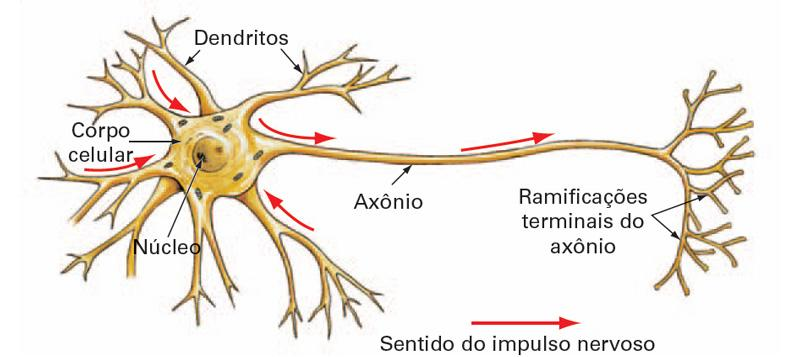
\includegraphics[scale=.7]{neuronio}
Fonte: o Autor
\end{figure}
\lstset{language=Python}
\begin{lstlisting}[frame=single, numbers=left, caption=Função]
def create_dataset(img_folder):

	img_data_array=[]
	class_name=[]

for dir1 in os.listdir(img_folder):
for file in os.listdir(os.path.join(img_folder, dir1)):

image_path= os.path.join(img_folder, dir1,  file)
# ajuste para ler em escala de cinza
#image= cv2.imread( image_path, cv2.COLOR_BGR2RGB)
image= cv2.imread( image_path, 0)
#print(image_path)
image=cv2.resize(image, (IMG_HEIGHT, IMG_WIDTH),interpolation = cv2.INTER_AREA)
image=np.array(image)
image = image.astype('float32')
image /= 255 
img_data_array.append(image)
class_name.append(dir1)

target_dict={k: v for v, k in enumerate(np.unique(class_name))}
for i in target_dict:
print(i)

#return img_data_array, class_name
matriz_rotulos = []
for i in class_name:
rotulo = target_dict[i]
matriz_rotulos.append(rotulo)

# for i in matriz_rotulos:
#     print(i)
return np.array(img_data_array, np.float32), np.array(list(matriz_rotulos), np.float32)	
\end{lstlisting}

\end{document}
